\documentclass{scrartcl}

\include{header/zusammenfassung}
\include{header/hyperref}

% tikz zeug
\usepackage{pgfplots}
\pgfplotsset{compat=newest}
\input{3dparty/tikz-dsp.sty}
\usetikzlibrary{chains}
\DeclareMathAlphabet{\mathpzc}{OT1}{pzc}{m}{it}
\newcommand{\z}{\mathpzc{z}}

\title{DigSig2 Zusammenfassung}
\author{Jürg Rast}

\begin{document}
\selectlanguage{english}
\setArrayStretch{2}
\maketitle
\newpage

\tableofcontents
\newpage

\section{Digital Filter Realizations\buch{Chapter 7}}

\subsection{Direct Form\buchSeite{265}}
\label{sec:directform}
Also called \emph{direct form I}. Consider a second-order filter with
transfer function
\begin{equation*}
	H(z) = \frac{N(z)}{D(z)} 
		 = \frac{b_0 + b_1z^{-1} + b_2z^{-2}}{1 + a_1z^{-1} + a_2z^{-2}}
\end{equation*}
with the I/O difference equation
\begin{equation*}
	y_n = -a_1 y_{n-1} - a_2 y_{n-2} + b_0 x_n + b_1 x_{n-1} b_2 x_{n-2}
\end{equation*}\\

This results in the following block diagram: \\

\begin{center}
	\input{tikz/DirectForm}
\end{center}

\subsection{Canonical Form\buchSeite{271}}
\label{sec:canonicalform}
The most popular form. Also called \emph{direct form II}. It can be obtained from
the \nameref{sec:directform} by splitting it up, introducing an intermediate signal $w(n)$ and reversing it.

\begin{align*}
	H(z) &= \frac{1}{D(z)} \cdot N(z) \\
	w(n) &= x(n) - a_1 w(n-1) - a_2 w(n-2) \\
	y(n) &= b_0 w(n) + b_1 w(n-1) + b_2 w(n-2) \\
\end{align*}\\

\begin{center}
	% FIR filter as block diagram
\begin{tikzpicture}
	% Place nodes using a matrix
	\matrix (m) [row sep=2.5mm, column sep=5mm]
	{
		%--------------------------------------------------------------------
		\node[dspnodeopen,dsp/label=above] (m00) {$x(n)$};    &
		\node[dspadder]                    (m01) {};          &
		\node[coordinate]                  (m02) {};     &
		\node[coordinate]                  (m03) {};          &
		\node[dspmixer, dsp/label=below]   (m04) {$b_0$};     &
		\node[dspadder]                    (m05) {};          &
		\node[dspnodeopen,dsp/label=above] (m06) {$y(n)$};    \\
	
		
		\node[coordinate]                  (m10) {};          &
		\node[coordinate]                  (m11) {};          &
		\node[coordinate]                  (m12) {};          &
		\node[dspsquare]                   (m13) {$\z^{-1}$}; &
		\node[coordinate]                  (m14) {};          &
		\node[coordinate]                  (m15) {};          &
		\node[coordinate]                  (m16) {};          \\
		
		\node[coordinate]                  (m20) {};          &
		\node[coordinate]                  (m21) {};          &
		\node[dspmixer, dsp/label=below]   (m22) {$-a_1$};     &
		\node[coordinate]                  (m23) {};          &
		\node[dspmixer, dsp/label=below]   (m24) {$b_1$};     &
		\node[coordinate]                  (m25) {};          &
		\node[coordinate]                  (m26) {};          \\
		
		
		\node[coordinate]                  (m30) {};          &
		\node[coordinate]                  (m31) {};          &
		\node[coordinate]                  (m32) {};          &
		\node[dspsquare]                   (m33) {$\z^{-1}$}; &
		\node[coordinate]                  (m34) {};          &
		\node[coordinate]                  (m35) {};          &
		\node[coordinate]                  (m36) {};          \\
		
		\node[coordinate]                  (m40) {};          &
		\node[coordinate]                  (m41) {};          &
		\node[dspmixer, dsp/label=below]   (m42) {$-a_2$};     &
		\node[coordinate]                  (m43) {};          &
		\node[dspmixer, dsp/label=below]   (m44) {$b_2$};     &
		\node[coordinate]                  (m45) {};          &
		\node[coordinate]                  (m46) {};          \\
		};
		
	% Draw connections
	\begin{scope}[start chain]
		\chainin (m00);
		\chainin (m01) [join=by dspconn];
		\chainin (m04) [join=by dspconn];
		\chainin (m05) [join=by dspconn];
		\chainin (m06) [join=by dspconn];
	\end{scope}
	
	\begin{scope}[start chain]
		\chainin (m03);
		\chainin (m13) [join=by dspconn];
		\chainin (m23) [join=by dspline];
		\chainin (m33) [join=by dspconn];
		\chainin (m43) [join=by dspline];
	\end{scope}
	
	\foreach \i in {2,4}
	{
		\begin{scope}[start chain]
			\chainin (m\i3);
			\chainin (m\i2) [join=by dspconn];
			\chainin (m01) [join=by dspconn];
		\end{scope}
	}
	
	\foreach \i in {2,4}
	{
		\begin{scope}[start chain]
			\chainin (m\i3);
			\chainin (m\i4) [join=by dspconn];
			\chainin (m05) [join=by dspconn];
		\end{scope}
	}
		
	\draw[] (m01) -- node[midway,above] {$w_0$} (m04);
	\draw[] (m23) -- node[midway,above] {$w_1$} (m24);
	\draw[] (m43) -- node[midway,above] {$w_2$} (m44);
\end{tikzpicture}
\end{center}

\subsection{Cascade Form\buchSeite{277}}
\label{sec:cascadeform}
For filters with real impulse responses (all $a_i$ and $b_i$ are real), the
transfer function can be written by cascaded 2nd order sections (SOS).

\begin{align*}
	H(z) = \prod_{i=0}^{K-1}H_i(z) = \prod_{i=0}^{K-1}\frac
	{b_{i0}+b_{i1}z^{-1}+b_{i2}z^{-2}}
	{1+a_{i1}z^{-1}+a_{i2}z^{-2}} &&
\end{align*}

Usually the SOS are implemented in the canonical form. A first order term is
implemented by setting the $z^{-1}$ term to zero. The advantage of the cascade
form is the efficient implementation of 2nd order sections in DSPs.

\subsection{Cascade $\Leftrightarrow$ Canonical\buchSeite{284}}
To find the \nameref{sec:cascadeform} of a filter, $D(z)$ and $N(z)$ are
factored into 2nd order sections. 

\begin{align*}
D(z) &= 1 + a_1 z^{-1} + a_2 z^{-2} + \dots + a_M z^{-M} &\\
&=(1-p_1z^{-1})(1-p_2z^{-1}) \dots (1-p_Mz^{-1})&
\end{align*}

For real-valued roots, any two factors can be combined:
\begin{equation*}
	(1 - p_1 z^{-1}) (1 - p_2 z^{-1}) = (1 - (p_1 + p_2) z^{-1} + p_1 p_2 z^{-2})
\end{equation*}

Conjugate complex roots are paired (if the coefficients are real):
\begin{equation*}
	(1 - p_1 z^{-1}) (1 - p_1^* z^{-1}) = 1 - 2 \text{Re}(p_1) z^{-1} + |p_1|^2 z^{-2}
\end{equation*}

\section{Signal Processing Applications\buch{Chapter 8}}
\subsection{Digital Waveform Generators}
\subsubsection{Sinusodial Generators}
\[
	h(n) = R^n \sin(\omega_0 n)u(n) \qquad
	H(z) = \frac{R \sin \omega_0 z^{-1}}{1-2R\cos \omega_0 z^{-1} + R^2 z^{-2}}
\]

\subsubsection{Periodic Waveform Generators}
In order for $x(n)$ to be periodic in the time index $n$ with some period, say of $D$ samples,
it is necessary that one whole period of the signal fit within the $D$ samples, that is,
at $n = D$ the signal must cycle by one whole period.

This requires that $x(D) = x(0)$, which requires
\[
	\omega = \frac{2\pi}{D} \qquad f = \frac{f_s}{D} \qquad f_s = D \qquad T_D = DT
\]

Because of the periodicity, it is enough to specifiy the signal over one period only:
\[
	h = [b_0, b_1, \ldots, b_{D-1}, b_0, b_1, \ldots, b_{D-1}, b_0, \ldots]
\]

With the corespondig z-Transformation:
\[
	H(z) = \frac{b_0 + b_1 z^{-1} + b_2 z^{-2} + \ldots + b_{D-1} z^{-(D-1)}}{1 - z^{-D}}
\]

\subsubsection{Wavetable Generators}

\subsection{Digital Audio Effects}
\begin{tabular}{|l|l|l|l|}
\hline 
\textbf{Filter} & \textbf{Signal} $y(n) = $ & 
\textbf{Transfer function} & \textbf{Impulse response} $ h(n) = $
\\ \hline
echo filter & $x(n) + ax(n-D)$ &
$H(z) = 1 + az^{-D}$ & $\delta(n) + a \delta(n-D)$
\\ \hline
plain reverberator & $a y(n-D) + x(n)$ &
$H(z) = \frac{1}{1-a z^{-D}}$ & $\delta(n) + a \delta(n-D) + a^2 \delta(n- 2D) + \ldots$
\\ \hline
allpass reverberator & $a y(n-D) -ax(n) + x(n-D)$ & $H(z) = \frac{-a + z^{-D}}{1-az^{-D}} $ &
\\ \hline
flanging processor & $x(n) + a x(n- d(n))$ & &
\\ \hline
\end{tabular}


\subsubsection{Multitab Delays}
\subsubsection{Compressors, Limiters, Expanders, and Gates}

\subsection{Noise Reduction and Signal Enhancement}

\subsubsection{Noise Reduction Filters\buchSeite{382-385}}
\begin{flalign}
&\text{noise measured Signal}&& x(n)=s(n)+\nu(n)&&&&\notag\\
&\text{desired signal}&& s(n)&&&&\notag\\ 
&\text{noise}&& \nu(n)&&&&\notag\\
& \text{noise reduction ration} && 
NRR=\frac{\sigma_{y_{\nu}}^2}{\sigma_{\nu}^2}
=\int\limits_{-\pi}^{\pi}|H(\omega)|^2 \frac{d\omega}{2\pi} =\sum_n h_n^2 &&&&\notag\\
& \text{Ideal Lowpass filter} && NRR=\frac{\sigma_{y_{\nu}}^2}{\sigma_{\nu}^2}
=\int\limits_{-\omega_c}^{\omega_c}1\frac{\omega}{2\pi}=\frac{2\omega_c}{2\pi}=\frac{\omega_c}{\pi} &&&&\notag\\
&\text{input mean-square noise}&&\sigma_{\nu}^2 &&&&\notag\\
&\text{output mean-square noise}&& \sigma_{y_{\nu}}^2 &&&&\notag\\
& \text{SNR and NRR ratio}&& \frac{SNR_{out}}{SNR_{in}}=\frac{1}{NRR}&&&&\notag
\end{flalign}

\subsubsection{Notch and Comb Filters\buchSeite{398-406}}
Two special cases of the signal enhancement/noise reduction problem arise when:
\begin{enumerate}

\item The noise signal v(n) in Eq. (8.3.1) is periodic. Its spectrum is concentrated at
the harmonics of a fundamental frequency. The noise reduction filter is an ideal
notch filter with notches at these harmonics \item The desired signal s(n) is periodic and the noise is a wideband signal. Now, the
signal enhancement filter is an ideal comb filter with peaks at the harmonics of
the desired signal
\end{enumerate} 

The ideal notch and comb filters are complementary filters,
in the sense that one is zero where the other is one, so that their frequency responses
add up to unity:

normalized to unity half-way between the notches:
\begin{flalign}
& H_{notch}(z)=\frac{bN(z)}{N(\rho z)}=b \frac{1-z^{-D}}{1-az{-D}}&& b=\frac{1+a}{2}&& a=\rho^D &&
\omega k = \frac{(2k + 1)\pi}{D} &&\notag\\
&&&&&&&\notag\\
& \text{paramter a on the desired 3-dB width:}&& \Delta\omega=\frac{2\pi\Delta f}{f_s}&&\text{on the notch dips}  &&\notag\\
&&&&&&&\notag\\
& &&\beta=\tan \frac{D\Delta\omega}{4} && a=\frac{1-\beta}{1+\beta} && b=\frac{1}{1+\beta}&&\notag\\
& \text{restriction and maximum value}&& 0<\beta<1 && \Delta\omega\leqslant\frac{\pi}{D}&& \Delta\leqslant\frac{f_s}{2D}&&\notag\\
&\text{squared magnitude response}&&\left|H_{notch}(\omega)\right|^2&&=\frac{\tan^2(\omega D /2)}{\tan^2(\omega D/2)+\beta^2}&&\notag
\end{flalign}


\emph{narrow lowpass filter:}
\begin{flalign}
& \text{normalized} && H_{comp}(z)=b \frac{1+z^{-D}}{1-az{-D}}&& b=\frac{1-a}{2}&& a=\rho^D &&&&\notag\\
&\text{peaks at} && \omega k = \frac{2k\pi}{D} && \text{zeros at}&&
\omega k = \frac{(2k + 1)\pi}{D} &&\notag\\
&&&&&&&\notag\\
& \text{paramter a on the desired 3-dB width:}&& \Delta\omega=\frac{2\pi\Delta f}{f_s}&&  &&\notag\\
&&&&&&&\notag\\
& &&\beta=\tan \frac{D\Delta\omega}{4} && a=\frac{1-\beta}{1+\beta} && b=\frac{\beta}{1+\beta}&&\notag\\
&\text{squared magnitude response}&&\left|H_{comb}(\omega)\right|^2&&=\frac{\beta^2}{\tan^2(\omega D/2)+\beta^2}&&\notag
\end{flalign}
\begin{flalign}
& H_{notch}(\omega)+H_{comb}(\omega)=\frac{1-a}{2}\frac{1+z^{-D}}{1-az^{-D}}+\frac{1+a}{2}\frac{1-z^{-D}}{1-az^{-D}}=1&&\notag
\end{flalign}




\subsubsection{Signal Averaging\buchSeite{421-425}}
The transfer function can be derived by taking a length N FIR averaging filter and applying the replication transform $z \rightarrow z^D$
\begin{flalign}
& H(z)=\frac{1}{N}\left( 1+ z{-D}+z{-2D}+\ldots + z{-(N-1)D} \right)=\frac{1}{N}\frac{z{-ND}}{1-z{-D}}&&\notag
\end{flalign}
In the time domain, the signal averaging comb filter is given by the following I/O difference equation
\begin{flalign}
& y(n)=\frac{1}{N}\left[x(n)+x(n-D)+x(n-2D)+\ldots+x(n-(N-1)D)\right] &&\notag
\end{flalign}
In general, that is there are N periods
\begin{flalign}
& \hat{y}(n)=\frac{1}{N}\sum_{i=0}^{N-1}x_i(n) && \hat{y}(n)=\frac{1}{N}\sum_{i=0}^{N-1}(s(n)+\nu_i(n))=s(n)+ \frac{1}{N}\sum_{i=0}^{N-1}\nu_i(n)=s(n)+\hat{\nu}(n)&&\notag\\
&\sigma_{\hat{\nu}}^2=\frac{1}{N^2}(\sigma_{\nu}^2+\sigma_{\nu}^2+\ldots+\sigma_{\nu}^2)=\frac{1}{N^2}(N\sigma_{\nu}^2)=\frac{1}{N}\sigma_{\nu}^2 &&&&\notag
\end{flalign}

\subsubsection{Savitzky-Golay Smoothing Filters\buchSeite{427-451}}

Lin-Alg matrices see book

\section{DFT- / FFT-Algorithms}

\subsection{DFT}
\subsubsection{Module-N reduction}
\begin{itemize}
	\item Opposite of zero padding
\end{itemize}

\subsection{IDFT}

\begin{equation}
	IDFT(X) = \frac{1}{N}\left[DFT(X^*)\right]^*
	\label{eq:IDFT}
\end{equation}


\section{FIR Digital Filter Design\buch{Chapter 10}}

\subsection{Windowing Methods}
\subsubsection{Ideal Filters}
\subsubsection{Rectangular Window}
\subsubsection{Hamming Window}

\subsection{Kaiser Window}
\begin{align*}
	\alpha = \left\{
		\begin{array}{l l}
			0.1102(A-8.7)& \quad \text{if } A \geq 50\\
			0.5842(A-21)^{0.4}+0.07886(A-21) & \quad \text{if }21 < A < 50\\
			0 & \quad \text{if } A \leq 21
		\end{array} \right.
\end{align*}
\subsubsection{Kaiser Window for Filter Design}


\textbf{Regeln:}\\
pass und stopp Band sind identisch, sind sie unterschiedlich vorgegeben muss die härtere Bedingung verwendet werden \\
\begin{align*}
\delta=min(\delta_{pass},\delta_{stop})
\end{align*}
schlussendlich wird der Filter in beiden Bändern die gleiche Überschreitung haben
\begin{align*}
A=-20log_{¶10}\delta && \delta=10^{-A/20}
\end{align*}
Das Stopp band hat meistens die strengeren Anforderungen
\subsubsection{Kaiser Window for Spectral Analysis}
\subsection{Frequency Sampling Method}

\subsection{Other FIR Design Methods}


\section{IIR Digital filter Design\buch{Chapter 11}}
\subsection{Bilinear Transformation}
Designflow:
\begin{center}
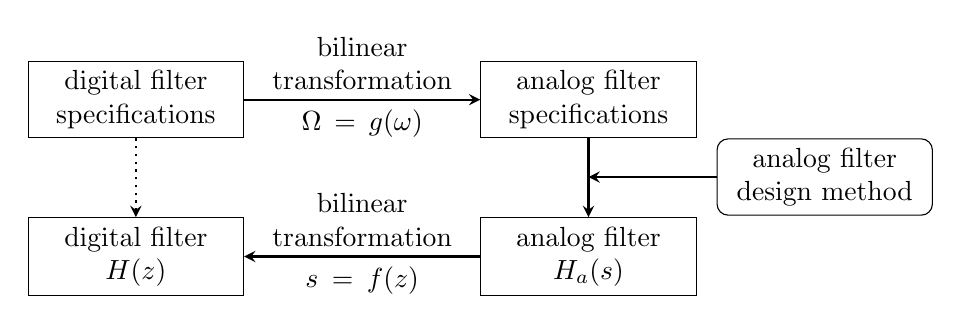
\begin{tikzpicture}[
	node distance=3cm,
	block/.style={text width=2.5cm,text centered
	}]
\node[draw, block] (dfs) {digital filter specifications};
\node[draw, block, right=of dfs] (afs) {analog filter specifications};
\node[draw, block, below=1cm of dfs] (df) {digital filter \\ $H(z)$};
\node[draw, block, below=1cm of afs] (af) {analog filter \\ $H_a(s)$};
\node[draw, block, below=0cm of afs, xshift=3cm, rounded corners] (afdm) {analog filter design method};

\draw[-stealth, thick] (dfs) -- (afs) 
	node[block, midway, above] {bilinear \\ transformation}
	node[block, midway, below] {$\Omega = g(\omega)$};
\draw[-stealth, thick, dotted] (dfs) -- (df);

\draw[-stealth, thick] (af) -- (df) 
	node[block, midway, above] {bilinear \\ transformation}
	node[block, midway, below] {$s = f(z)$};
\draw[-stealth, thick] (afs) -- (af);

\draw[-stealth, thick] (afdm) -- +(-3,0);
\end{tikzpicture}
\end{center}
Maps from z-plane to the s-plane (from the analog frequency to the digital
frequency)

\begin{tabularx}{\textwidth}{|l|X|X|}
	\hline
	\textbf{Filter} & \textbf{bilinear transformation} & \textbf{frequency map}
	\\ \hline
	lowpass & 
	$s = f(z) = \frac{1 - z^{-1}}{1 + z^{-1}}$ &
	$ \Omega = g(\omega) = \tan(\frac{\omega}{2})$
	\\ \hline
	highpass & 
	$s = f(z) = \frac{1 + z^{-1}}{1 - z^{-1}}$ &
	$ \Omega = g(\omega) = - \cot(\frac{\omega}{2})$
	\\ \hline
	bandpass & 
	$s = f(z) = \frac{1 - 2cz^{-1} z^{-2}}{1 + z^{-2}}$ &
	$ \Omega = g(\omega) = \frac{c - \cos(\omega)}{\sin(\omega)}$
	\\ \hline
	bandstop & 
	$s = f(z) = \frac{1 + z^{-2}}{1 - 2cz^{-1} z^{-2}}$ &
	$ \Omega = g(\omega) = \frac{\sin(\omega)}{\cos(\omega) - c}$ 
	\\ \hline
\end{tabularx}

\subsection{First-Order Lowpass and Highpass Filters}
Lowpass:
\begin{align}
	H(z) &= \frac{b_0 + b_1 z^{-1}}{1+a_1 z^-1}\\
	\omega_c &= \frac{2 \pi f_c}{f_s}\\
	|H(\omega_c)|^2 &= \frac{1}{2}
\end{align}
\subsection{Second-Order Peaking and Notching Filters}
\subsection{Parametric Equalizer Filters}
\subsection{Comb Filters}

\subsection{Higher Order Filters}
\subsubsection{Analog Lowpass Butterworth Filters}
\subsubsection{Digital Lowpass Filters}
\subsubsection{Digital Highpass Filters}
\subsubsection{Digital Bandpass Filters}
\subsubsection{Digital Bandstop Filters}
\subsubsection{Chebyshev Filter Design}

%!TEX root = ../DigSig2.tex
\section{Interpolation, Decimation and Oversampling\buch{Chapter 12}}
\subsection{Interpolation and Oversampling\buchSeite{632-637}}
Oversampling is increasing the sample rate and requires some form of interpolation. New samples at a higher sampling rate are created. These are calculated using a FIR filter. The spectrum of the low-rate and the high-rate signal are identical, if the frequency axis is not normalized.

\subsection{Interpolation Filter Design\buchSeite{638-657}}
\subsubsection{Direct form\buchSeite{638}}

\begin{center}
	\includegraphics[width=10cm]{images/IntDecOv_IncSamplingRate.jpg}
\end{center}

There are now two discrete times, a fast one $n'$ and a slow one called $n$.
The effect on the spectrum of a signal and the advantage in DA-Conversion is
shown in the following figure (left: original spectrum, right: spectrum
at high rate).

\begin{center}
	\includegraphics[width=16cm]{images/IntDecOv_Spectrum.jpg}
\end{center}

The Job of the FIR filter is to move the zeros to the appropriate values,
or to erase the spectral copies of the original spectrum in the new
Nyquist band. \\

\begin{center}
	\includegraphics[width=8cm]{images/IntDecOv_Filter.jpg}
\end{center}

The ideal lowpass filter for an $L$-fold interpolation is operating at the fast
sampling rate $f'_s=L f_s$ and has its cutoff frequency at the low-sampling
rate's Nyquist frequency $f_s/2$.

\begin{equation*}
	f_c = \frac{f_s}{2}=\frac{f'_s}{2L}
	\qquad
	\omega'_c = \frac{2\pi f_c}{f'_s}=\frac{\pi}{L}
\end{equation*}

\begin{tabularx}{\linewidth}{Xl}
	FIR approximation to the ideal interpolator (non causal):
	& $d(k')=\frac{\sin(\pi k'/L)}{\pi k'/L}$, with $-LM\leq k'\leq LM$\\
	By delaying this filter by $LM$ samples, it gets causal:
	& $h(n')=d(n'-LM)=\frac{\sin(\pi (n'-LM)/L)}{\pi (n'-LM)/L}$ \\
	Using a Hamming window: & $h(n')=w(n')d(n'-LM)$ \\
	Hamming window & $w(n') = 0.54-0.46\cos(\frac{2\pi n'}{N-1})$ \\
\end{tabularx} \\

The output of the non causal FIR interpolator filter is obtained as the
convolution of the upsampled signal with the filter

\begin{equation*}
	y_{up}(n') = \sum\limits_{k'=-LM}^{LM}d(k')x_{up}(n'-k')
\end{equation*}


\subsubsection{Polyphase Form\buchSeite{640}}

\begin{multicols}{2}
	The direct form is
	\begin{center}
		\adjustbox{max width=0.7\linewidth}{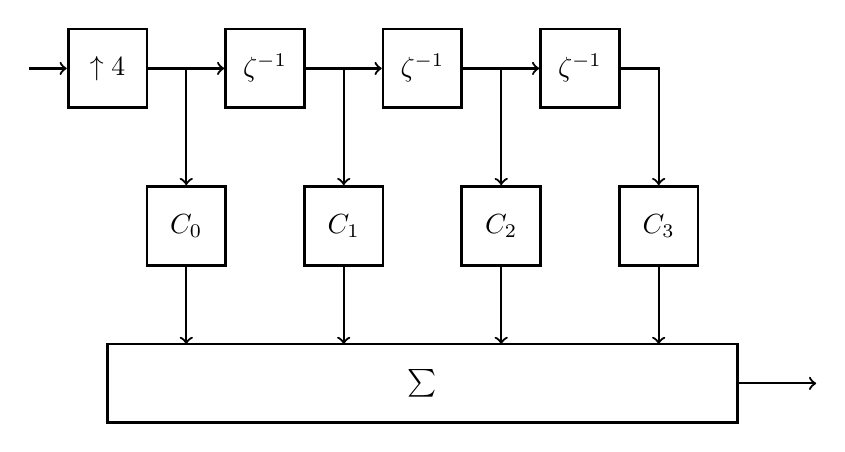
\begin{tikzpicture}
[	
	sq/.style={rectangle,draw,line width=1,minimum height=1cm,minimum width=1cm}
]

\node[sq] (t1) at (1,0) {$\zeta^{-1}$};
\node[sq] (t2) at (3,0) {$\zeta^{-1}$};
\node[sq] (t3) at (5,0) {$\zeta^{-1}$};

\node[sq] (c1) at (0,-2) {$C_0$};
\node[sq] (c2) at (2,-2) {$C_1$};
\node[sq] (c3) at (4,-2) {$C_2$};
\node[sq] (c4) at (6,-2) {$C_3$};

\node[rectangle,draw,line width=1,minimum height=1cm, minimum width=8cm] (sum) at (3,-4) {$\sum$};
\node[sq] (ds) at (-1,0) {$\uparrow 4$};

\draw[thick,->]	(ds)	-- 	(t1);
\draw[thick,->]	(t1)		-- 	(t2);
\draw[thick,->]	(t2) 		-- 	(t3);

\draw[thick,->] (ds)	-|	(c1);
\draw[thick,->] (t1)		-|	(c2);
\draw[thick,->] (t2)		-|	(c3);
\draw[thick,->] (t3)		-|	(c4);

\draw[thick,->] (c1) 		-- 	(0,-3.5);
\draw[thick,->] (c2) 		-- 	(2,-3.5);
\draw[thick,->] (c3) 		-- 	(4,-3.5);
\draw[thick,->] (c4) 		-- 	(6,-3.5);

\draw[thick,->] (-2,0) -- (ds);
\draw[thick,->] (sum) -- (8,-4);


\end{tikzpicture}}
	\end{center}
\vfill\columnbreak
	A more efficient way is using the polyphase form
	\begin{center}
		\adjustbox{max width=\linewidth}{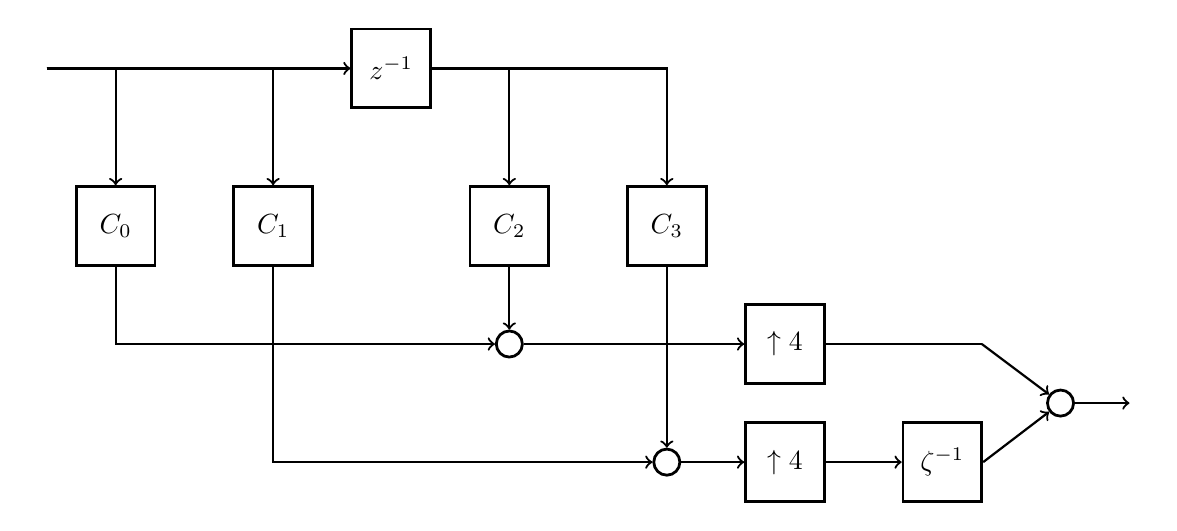
\begin{tikzpicture}
[	
	sq/.style={rectangle,draw,line width=1,minimum height=1cm,minimum width=1cm},
	rd/.style={circle,draw,line width=1,radius=0.5cm}
]

\node[sq] (t1) at (3.5,0) {$z^{-1}$};

\node[sq] (c1) at (0,-2) {$C_0$};
\node[sq] (c2) at (2,-2) {$C_1$};
\node[sq] (c3) at (5,-2) {$C_2$};
\node[sq] (c4) at (7,-2) {$C_3$};

\node (start) at (-1,0) {};

\draw[thick,->] (start) -| (c1);
\draw[thick,->] (start) -| (c2);
\draw[thick,->] (start) -- (t1);
\draw[thick,->] (t1) -| (c3);
\draw[thick,->] (t1) -| (c4);

\node[rd] (s1) at (5,-3.5) {};
\node[rd] (s2) at (7,-5) {};

\draw[thick,->] (c1) |- (s1);
\draw[thick,->] (c3) -- (s1);
\draw[thick,->] (c2) |- (s2);
\draw[thick,->] (c4) -- (s2);

\node[sq] (us1) at (8.5,-3.5) {$\uparrow 4$};
\node[sq] (us2) at (8.5,-5) {$\uparrow 4$};

\draw[thick,->] (s1) -- (us1);
\draw[thick,->] (s2) -- (us2);

\node[sq] (t2) at (10.5,-5) {$\zeta^{-1}$};
\draw[thick,->] (us2) -- (t2);

\node[rd] (s3) at (12,-4.25) {};
\node (p1) at (11,-3.5) {};

\draw[thick] (us1) -- (p1.center);
\draw[thick,->] (p1.center) -- (s3);
\draw[thick,->] (t2.east) -- (s3);

\node (end) at (13,-4.25) {};
\draw[thick,->] (s3) -- (end);

\end{tikzpicture}}
	\end{center}
\end{multicols}

Note that the direct form does all multiplications at the high rate, while
the polyphase form allows doing the multiplications at the low rate, which
makes the system more efficient. \\

Suppose the low-rate time instants are $n$, then the fast-rate time instants
can be described as $n' = NL+i$ for $i=0,1,\ldots,L-1$. The output is therefore

\begin{equation*}
	y_{up}(nL+i) = \sum\limits_{k=-M}^{M-1}\sum\limits_{j=0}^{L-1} d(kL+j) x_{up}(nL+i-kL-j)
\end{equation*}

which allows us to split the output $y_{up}$ into $y_i(n)=y_{up}(nL+i)$.
We can also define the \emph{$i$th polyphase subfilter} as

\begin{equation*}
	d_i(k) = d(kL+i) \:,\qquad -M \leq k \leq M-1 \:,\quad i=0,1,\ldots,L
\end{equation*}

The $i$th outputs can now be calculated in terms of the slow-rate samples

\begin{equation*}
	y_i(n) = \sum\limits_{k=-M}^{M-1}d_i(k) x(n-k) \:,\qquad i=0,1,\ldots,L-1
\end{equation*}

The output $y_{up}$ is now only calculated in terms of the slow sampling rate,
which decreases the computational rate in terms of multiplications per second by
a factor of $L$, from $R = NLf_s$ (direct from) to $R = Nf_s$ (polyphase form).


\subsubsection{Frequency domain characteristics\buchSeite{645}}
To discuss the interpolation in the frequency domain, we introduce the different
unit delays $z$ (low sampling rate = long delay) and $\zeta$
(high sampling rate = short delay)

\begin{equation*}
	z = \zeta^L \qquad \Leftrightarrow \qquad \zeta = z^{1/L}
\end{equation*}

The high-rate output can now be written in the $z$-Domain as

\begin{equation*}
	Y_{up}(\zeta) = \sum\limits_{i=0}^{L-1} \zeta^{-i} Y_i(\zeta^L)
	= \sum\limits_{i=0}^{L-1} z^{-i/L} Y_i(z)
\end{equation*}

which is what we already know from the time domain. The filter $D(\zeta)$
similarly is

\begin{equation*}
	D(\zeta) = \sum\limits_{i=0}^{L-1} \zeta^{-i} D_i(\zeta^L)
	= \sum\limits_{i=0}^{L-1} z^{-i/L} D_i(z)
\end{equation*}

The 0th polyphase subfilter $d_0(k)$ should of course return the same value as
the input $x(n)$, so the impulse response must be a dirac:
$d_0(k) = d(kL) = \delta(k)$. \\

The ideal filter which removes all spectral copies would generally have
the following characteristics
\begin{equation*}
	D(f) = \begin{cases}
		L\:,	& \text{if} \quad |f|\leq\frac{f_s}{2} \\
		0\:,	& \text{if} \quad \frac{f_s}{2}\leq |f|\leq\frac{f'_s}{2}
	\end{cases}
\end{equation*}

The ideal reconstructor $d(k)$, running at the higher rate $f_s'$ would
therefore be
\begin{equation*}
	d(k') = \frac{\sin(\pi k' / L)}{\pi k' / L}
\end{equation*}

This reconstructor is usually implemented using a Kaiser window design.

\subsection{Linear and Hold Interpolators\buchSeite{657-661}}
The reconstructor described above is the ideal interpolator. Nevertheless
there exist simpler interpolators, such as the linear and the hold interpolators.
Not surprising, these are not as good as the ideal interpolator, but especially
at high sample rates, the advantage of less calculations overweights the
downsides.

\subsubsection{Hold Interpolator}
\begin{multicols}{2}
	\begin{align*}
		d(k') &= \begin{cases}
			1\:, & \text{if} \quad 0\leq k' \leq L -1\\
			0\:, & \text{otherwise}
		\end{cases} \\
		y_{up}(nL+i) &= x(n) \\
		D(f) &= \frac{\sin(\pi f/f_s)}{\sin(\pi f/Lf_s)}e^{-j\pi(L-1)f/(Lf_s)}
	\end{align*}

	The polyphase subfilters $d_i(k)$ will then be

	\begin{equation*}
		d_i(k) = \delta(k)
	\end{equation*}

\vfill
\columnbreak
	\begin{center}
		\includegraphics[width=5cm]{images/IntDecOv_Hold.jpg}
	\end{center}
\vfill
\end{multicols}

\subsubsection{Linear Interpolator}
\begin{multicols}{2}
	\begin{align*}
		d(k') &= \begin{cases}
			1-\frac{|k'|}{L}\:, & \text{if} \quad |k'|\leq L -1\\
			0\:, & \text{otherwise}
		\end{cases} \\
		y_{up}(nL+i) &= (1-\frac{i}{L})x(n)+\frac{i}{L}x(n+1) \\
		D(f) &= \frac{1}{L}\left|\frac{\sin(\pi f/f_s)}{\sin(\pi f/Lf_s)}\right|^2
	\end{align*}

	The polyphase subfilters $d_i(k)$ will then be

	\begin{equation*}
		d_i(k) = (1-\frac{i}{L}) \delta(k) + \frac{i}{L} \delta(k+1)
	\end{equation*}
\vfill
\columnbreak
	\begin{center}
		\includegraphics[width=0.8\linewidth]{images/IntDecOv_Linear.jpg}
	\end{center}
\vfill
\end{multicols}


\subsection{Design Examples\buchSeite{661-686}}
%TODO!!!!
\subsubsection{4-fold interpolators\buchSeite{661}}
\begin{equation*}
  L = 4
\end{equation*}
with polyphase filter length $2M=4$ or $M=2$ which leads to a filter length $N=2LM+1=17$.
The ideal impulse response is:
\begin{equation*}
  d(k')=\frac{sin(\pi k'/4)}{\pi k'/4}, \qquad -8 \leq k' \leq 8
\end{equation*}
or, numerically,
\begin{equation*}
  \mathbf{h} = \mathbf{d} = [0, -0.13, -0.21, -0.18, 0, 0.30, 0.64, 0.90, 1, 0.90, 0.64, 0.30, 0, -0.18, -0.21, -0.13, 0]
\end{equation*}
where $\mathbf{h}$ is the causal version, and $\mathbf{d}$ is the symmetric one with time origin at the middle of the vector.
The resulting polyphase subfilters
\begin{equation*}
  d_i(k) = d(4k + i), \qquad -2 \leq k \leq 1
\end{equation*}
can now be calculated (high-rate filter subsampled by a factor of 4 and an increasing offset)
\begin{align*}
  \mathbf{h}_0 &= \mathbf{d}_0 = [0, 0, 1, 0] \\
  \mathbf{h}_1 &= \mathbf{d}_1 = [-0.13, 0.30, 0.90, -0.18] \\
  \mathbf{h}_2 &= \mathbf{d}_2 = [-0.21, 0.64, 0.64, -0.21] \\
  \mathbf{h}_2 &= \mathbf{d}_3 = [-0.18, 0.90, 0.30, -0.13]
\end{align*}
\begin{center}
  \includegraphics[width=6cm]{images/IntDecOv_DesignExample.png}
\end{center}
The interpolated samples $y_{\text{up}}(4n+i)$ between $x(n)=x_{\text{up}}(4n)$ and $x(n+1)=x_{\text{up}}(4[n+1])$ are now:
\begin{equation*}
  \begin{bmatrix}
    y_{\text{up}}(4n) \\
    y_{\text{up}}(4n+1) \\
    y_{\text{up}}(4n+2) \\
    y_{\text{up}}(4n+3)
  \end{bmatrix}
  =
  \begin{bmatrix}
        0 &    0 &    1 &     0 \\
    -0.13 & 0.30 & 0.90 & -0.18 \\
    -0.21 & 0.64 & 0.64 & -0.21 \\
    -0.18 & 0.90 & 0.30 & -0.13 \\
  \end{bmatrix}
  \begin{bmatrix}
    x_{\text{up}}(4n+8) \\
    x_{\text{up}}(4n+4) \\
    x_{\text{up}}(4n) \\
    x_{\text{up}}(4n-4)
  \end{bmatrix}
\end{equation*}
\begin{center}
  \includegraphics[width=8cm]{images/IntDecOv_DesignExampleSuperposition.png}
\end{center}

The 17 sample long FIR filter is very short ($M=2$).
This and the rectangular window have the effect that the interpolated signal is of low quality.
Rectangular windows should not be used, Hamming is much better and results in a reasonable interpolation even with $M=2$

The Hamming windowed version is obtained by multiplying the high-rate 17 sample long filter with the appropriate Hamming window resulting in
\begin{equation*}
  \begin{bmatrix}
    y_{\text{up}}(4n) \\
    y_{\text{up}}(4n+1) \\
    y_{\text{up}}(4n+2) \\
    y_{\text{up}}(4n+3)
  \end{bmatrix}
  =
  \begin{bmatrix}
        0 &    0 &    1 &     0 \\
    -0.02 & 0.22 & 0.87 & -0.07 \\
    -0.05 & 0.55 & 0.55 & -0.05 \\
    -0.07 & 0.87 & 0.22 & -0.02 \\
  \end{bmatrix}
  \begin{bmatrix}
    x_{\text{up}}(4n+8) \\
    x_{\text{up}}(4n+4) \\
    x_{\text{up}}(4n) \\
    x_{\text{up}}(4n-4)
  \end{bmatrix}
\end{equation*}
The resulting magnitude response shows, that the rectangular filter is steeper, at the high cost of 8.9\% overshoot, which the Hamming window version doesn't have.\\

For a block diagram realization of the polyphase form, recall these two relationships:
\begin{align*}
  Y_{\text{up}}(\xi) &= \sum_{i=0}^{L-1}\xi^{-1}Y_i(\xi^L) = \sum_{i=0}^{L-1}z^{-i/L}Y_i(z) \\
  D(\xi) &= \sum_{i=0}^{L-1}\xi^{-1}D_i(\xi^L) = \sum_{i=0}^{L-1}z^{-i/L}D_i(z)
\end{align*}
Therefore the transfer function of the high-rate interpolator filter can be written as the sum of the polyphase subfilters appropriately delayed:
\begin{align*}
  H(\xi) &= H_0(\xi^4) + \xi^{-1}H_1(\xi^4) + \xi^{-2}H_2(\xi^4) + \xi^{-3}H_3(\xi^4) \\
  &= H_0(z) + z^{-1/4}H_1(z) + z^{-2/4}H_2(z) + z^{-3/4}H_3(z)
\end{align*}
The resulting block diagram clearly shows how the four polyphase filters create the four output values.
Three of these values are interpolated while value $y_{\text{up}}(n') = y_{\text{up}}(4n) = y_0(n)$ is identical to the upsampled input value $x_{\text{up}}(n') = x_{\text{up}}(4n) = x(n)$, since $h_0=[0,0,1,0]$.
Clearly, the four output samples can be calculated in parallel, allowing for a very fast implementation.
\begin{center}
  \begin{tikzpicture}
    \node [inner sep=0pt,above right]
    {\includegraphics[width=10cm]{images/IntDecOv_DesignExamplePolyphase.png}};
    \draw[red,->] (9,7) node [right] {Missing upsampler by a factor of 4} -- (6,6.65) node {};
    \draw[red,->] (9,7) node {} -- (6,4.7) {};
    \draw[red,->] (9,7) node {} -- (6,2.75) {};
    \draw[red,->] (9,7) node {} -- (6,0.85) {};
  \end{tikzpicture}
\end{center}

\subsection{Decimation and Oversampling\buchSeite{686-691}}
Decimation is the inverse of oversampling, thus the sampling rate is reduced
from a high rate $f_s'$ to a low rate $f_s = f_s' / L$.

\begin{center}
	\includegraphics[width=10cm]{images/IntDecOv_Downsampler.jpg}
\end{center}

Downsampling is simply the process of discarding $L-1$ samples:

\begin{equation*}
	x_{down}(n) = \left.x'(n')\right|_{n'=nL} = x'(nL)
\end{equation*}

Caution: if the high rate spectrum occupies more than the low rate Nyquist rate
there \emph{will} be aliasing. \\

The ideal \emph{decimator} therefore contains a decimation filter, which
operates at the high frequencies and cuts out the low rate Nyquist band.

\begin{center}
	\includegraphics[width=12cm]{images/IntDecOv_Decimator.jpg}
\end{center}

The decimation filter is similar to the interpolation filter, except that
its DC gain is unity instead of $L$. A length-$N$ FIR decimation filter
can therefore be obtained by

\begin{equation*}
	h(n') = w(n') d(n'-LM) \:,\qquad \text{where} \quad
	d(k') = \frac{\sin(\pi k'/L)}{\pi k'}
\end{equation*}

Since only every $L$th output sample is needed, the filter output does
not need to be calculated for every fast rate sample (like on the left image),
reducing the computational cost by a factor $L$ to
$R = \frac{1}{L} N f_s' = N f_s$ (left image). \\

\begin{multicols}{2}
	\begin{center}
		\adjustbox{max width=0.9\linewidth}{\input{tikz/decimation}} \\
	\end{center}
\vfill\columnbreak
	\begin{center}
		\adjustbox{max width=0.7\linewidth}{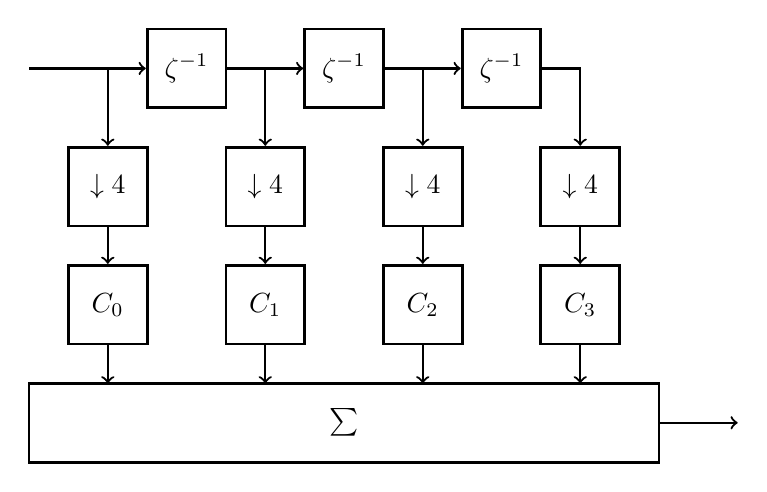
\begin{tikzpicture}
[	
	sq/.style={rectangle,draw,line width=1,minimum height=1cm,minimum width=1cm}
]

\node[sq] (t1) at (1,0) {$\zeta^{-1}$};
\node[sq] (t2) at (3,0) {$\zeta^{-1}$};
\node[sq] (t3) at (5,0) {$\zeta^{-1}$};

\node[sq] (d1) at (0,-1.5) {$\downarrow 4$};
\node[sq] (d2) at (2,-1.5) {$\downarrow 4$};
\node[sq] (d3) at (4,-1.5) {$\downarrow 4$};
\node[sq] (d4) at (6,-1.5) {$\downarrow 4$};

\node[sq] (c1) at (0,-3) {$C_0$};
\node[sq] (c2) at (2,-3) {$C_1$};
\node[sq] (c3) at (4,-3) {$C_2$};
\node[sq] (c4) at (6,-3) {$C_3$};

\node[rectangle,draw,line width=1,minimum height=1cm, minimum width=8cm] (sum) at (3,-4.5) {$\sum$};


\draw[thick,->]	(-1,0)	-- 	(t1);
\draw[thick,->]	(t1)		-- 	(t2);
\draw[thick,->]	(t2) 		-- 	(t3);

\draw[thick,->] (-1,0)	-|	(d1);
\draw[thick,->] (t1)		-|	(d2);
\draw[thick,->] (t2)		-|	(d3);
\draw[thick,->] (t3)		-|	(d4);

\draw[thick,->]	(d1)		-- 	(c1);
\draw[thick,->]	(d2)		-- 	(c2);
\draw[thick,->]	(d3)		-- 	(c3);
\draw[thick,->]	(d4)		-- 	(c4);

\draw[thick,->] (c1) 		-- 	(0,-4);
\draw[thick,->] (c2) 		-- 	(2,-4);
\draw[thick,->] (c3) 		-- 	(4,-4);
\draw[thick,->] (c4) 		-- 	(6,-4);

\draw[thick,->] (sum) -- (8,-4.5);

\end{tikzpicture}} \\
	\end{center}
\end{multicols}

Multistage designs are very popular for decimation filters. The early filters will
then be fast but simple, while later filters are slow but very precise. For fast
signals, often a simple FIR averaging filter is used. The last, slowest filter
can then be designed to fix the overall frequency response.


\subsection{Noise Shaping Quantizer\buchSeite{698-705}}

\paragraph{First-order delta-sigma A/D converters}
For first order delta-sigma A/D converters, only one bit is used: $B'=1$. For
slow signals, the quantization error will be small. The system will therefore
be oversampled such that the quantization noise is moved into higher frequencies,
which are then suppressed by the digital decimation filter.

\begin{center}
	\includegraphics[width=11cm]{images/IntDecOv_SigmaDelta.jpg}
\end{center}

To be able to create a discrete time model, we replace the quantizer by
an additive quantization noise model.

\begin{center}
	\includegraphics[width=10cm]{images/IntDecOv_SigmaDeltaModel.jpg}
\end{center}

The transfer functions for the input $X$ and the noise $NS$ will then be

\begin{equation*}
	H_X(\zeta) = \zeta^{-1} \qquad H_{NS}(\zeta) = 1 - \zeta^{-1}
\end{equation*}

or for higher orders $p$: $H_{NS}(\zeta) = (1-\zeta^{-1})^p$. \\

The MSE is obtained by
\begin{equation*}
  \sigma_e^2 = \sigma_{e'}^2 \frac{1}{f_s^{'}} \int_{-f_s/2}^{f_s/2} |H_{NS}(f)|^2 df
\end{equation*}
with $f_s^{'} = L f_s$ and
\begin{equation*}
  |H_{NS}(f)|^2 = |2 \sin(\frac{\pi f}{f_s^{'}})|^{2p}
\end{equation*}

This leads to the known relationship of

\begin{equation*}
	\Delta B = (p+0.5) \log_2 L - 0.5 \log_2\left(\frac{\pi^{2p}}{2p+1}\right)
\end{equation*}


\paragraph{Oversampled noise shaping requantizers for D/A conversion}
Similarly, noise shaping and oversampling can be used for D/A conversion.

\begin{center}
	\includegraphics[width=12cm]{images/IntDecOv_Requantizer.jpg}
\end{center}

Again, using a discrete time model and a linear stochastic quantization
noise source, one gets to the following transfer functions for first-order
or higher-order noise shaping filters

\begin{align*}
	H(\zeta) &= \zeta^{-1} \qquad &
	H_{NS}(\zeta) &= (1-\zeta^{-1}) \qquad
	& \text{first-order} \\
	H(\zeta) &= 2 \zeta^{-1} - \zeta^{-2} \qquad &
	H_{NS}(\zeta) &= (1-\zeta^{-1})^2 \qquad
	& \text{second-order}
\end{align*}

and again

\begin{equation*}
	\Delta B = (p+0.5) \log_2 L - 0.5 \log_2\left(\frac{\pi^{2p}}{2p+1}\right)
\end{equation*}



\end{document}

